\documentclass{article}
\usepackage[en]{ukon-infie}
\usepackage[utf8]{inputenc}
\usepackage{algorithm2e}
\usepackage{amsmath}
\usepackage{graphicx}
% kann de oder en sein
% kann bubble break, topexercise sein

\Names{Jonas Probst, Simon Giebenhain}
\Lecture[AnaVis]{Analyse und Visualisierung von Informationen}
\Term{WS 2017/18}

\begin{document}
    \begin{ukon-infie}[5.12.17]{6}

        \begin{exercise}[p=7]{Cluster Summary}      
       \question{}
       {
       \textbf{k-Means:}
       \begin{enumerate}
       \item Even if the inital centroids are perfectly chosen,the smaller bottom clusters steal some points from the big one.
       \item This works fine, since the distances between the clusters are very big and they roughly contain an equal number of points
       \item If the inital location is perfect the result will be ok, but of course noise will also be assigned to some clusters. However if for example 2 inital centroids are in the top right cluster and the last inital centroid lies between the two remaining clusters, the top cluster will be split and the 2 bottom clusters will be merged.
       \end{enumerate}
       
      	\textbf{Hierarchical Clustering (Single Linkage):}
      	\begin{enumerate}
      	\item Works fine, because the distances between the clusters are bigger than the maximum distance within the clusters.
      	\item Works fine, because the distances between the clusters are bigger than the maximum distance within the clusters.
      	\item Depends on how the clusters are chosen from the hierarchical structure. If one cuts the branches at different heights, the desired results can be achieved. However if one cuts horizontally, either the upper right cluster will be bigger than indicated with the red circles or the bottom two clusters will not be there yet. This happens because the density in the bottom clusters is similar to the noise surrounding the top cluster.
      	\end{enumerate}
      	\textbf{DBSCAN:}
      	\begin{enumerate}
      	\item With sensible parameters, DBSAN will deliver a good result.
      	\item With sensible parameters, DBSAN will deliver a good result.
      	\item Because the density of the noise around the upper cluster is as high as the density of the bottom two clusters, DBSCAN will not work.
      	\end{enumerate}
      	
      	\textbf{OPTICS:}
      	\begin{enumerate}
      	\item 
      	\item
      	\item
      	\end{enumerate}
       }
              
       \question{}
       {
       \textbf{k-Means:}\\
       k can be chosen. If k deviates from 3, the result will be wrong.\\
       
       \textbf{Hierarchical Clustering(single linkage):}\\
       No parameters have to be chosen.\\
       
       
       \textbf{DBSCAN:}\\
		minPoints and $\epsilon$ have to be chosen.\\
		If minPoints is chosen too big, clusters with lower density will disapper.\\
		Similarily if minPoints is chosen too small, Clusters might merge with noise or other clusters (of course this also deoends on $\epsilon$).\\
		If $\epsilon$ is chosen too big, some clusters might merge and some clusters might absorb some noise.\\
		If $\epsilon$ is chosen too small, lower density clusters might disappear.\\
		In the example above Case 3 is especially affected form these parameters. If $\epsilon$ is rather small and minPoints is rather big, only the top cluster will be identified. The outher points constitue the noise cluster.\\
		If however $\epsilon$ is rather big and minPoints rather small, the bottom 2 clusters will be clustered correctly, but the top cluster will absorb the dense noise around it.
		
       
       \textbf{OPTICS:}\\
       }
       

		\end{exercise}
		
		\begin{exercise}[p=10]{K-Means}
		
		\end{exercise}
		
		


		\begin{exercise}[p=6]{DBSAN}
		{
		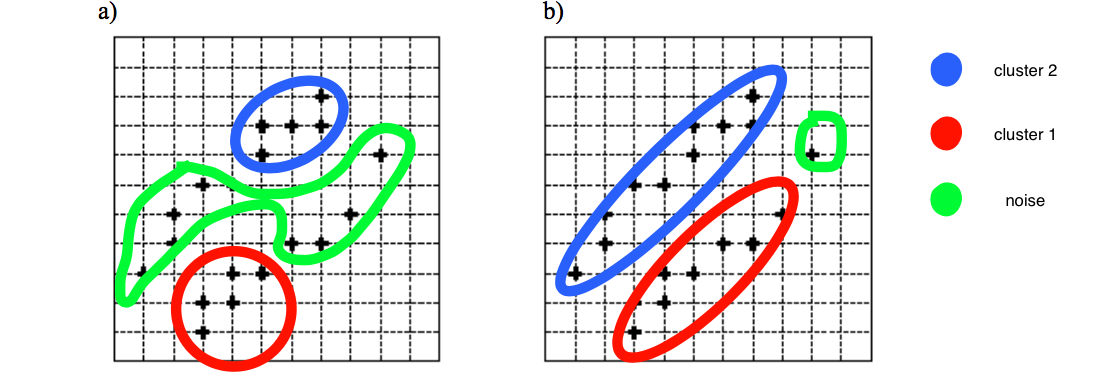
\includegraphics[scale=0.4]{dbscan.png}
		}
	
		\end{exercise}
		
		\begin{exercise}[p=3]{theoretical DBSAN}
		{
		They will belong to the first cluster, from wich the point is density-reachable, because in expand\_clusters() only unclassifed and noise points are added to the cluster. However in the unlikly event that the point is in the neighbourhood of a point, which initially expands a new cluster, the point will be reassigned to that clsuter.\\
		
		The first issue can be tackled, if instead of only considering unclassified and noise points, in the case a point is already assigned to another cluster, one computes the neighbourhood of that point and assignes the majority cluster in the neighbourhood to that point. In the case of a draw, one assignes the cluster with minimum distance to the point.\\
		
		The second issue can be tackled if one doen't blindly assign the new cluster to all point in the seed set, but checks wheter they are already assigned to some other class. In that cas proceed as explained above.
		}
	
		\end{exercise}
		
		
\end{ukon-infie}
\end{document}
